\subsection{Schema generale UC1}
\begin{figure}[H]
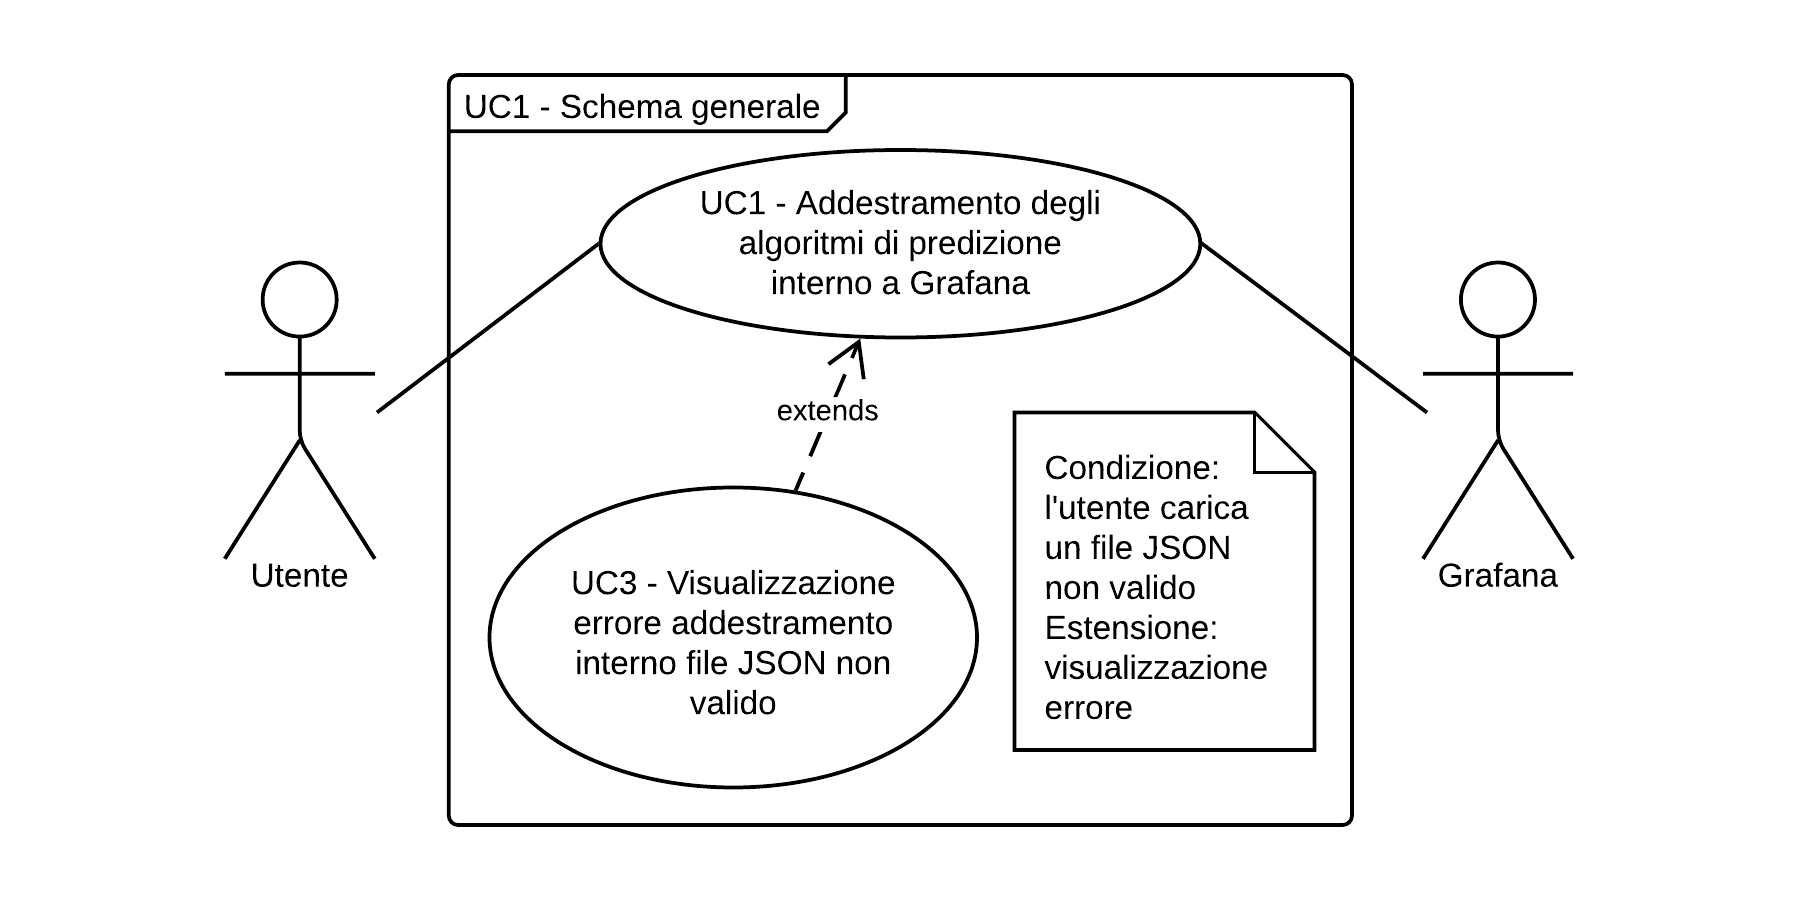
\includegraphics{img/UC1_-_Schema_generale.png}
\caption{Schema generale UC1}
\end{figure}
\subsection{UC1 - Addestramento degli algoritmi di predizione interno a Grafana}
\begin{figure}[H]
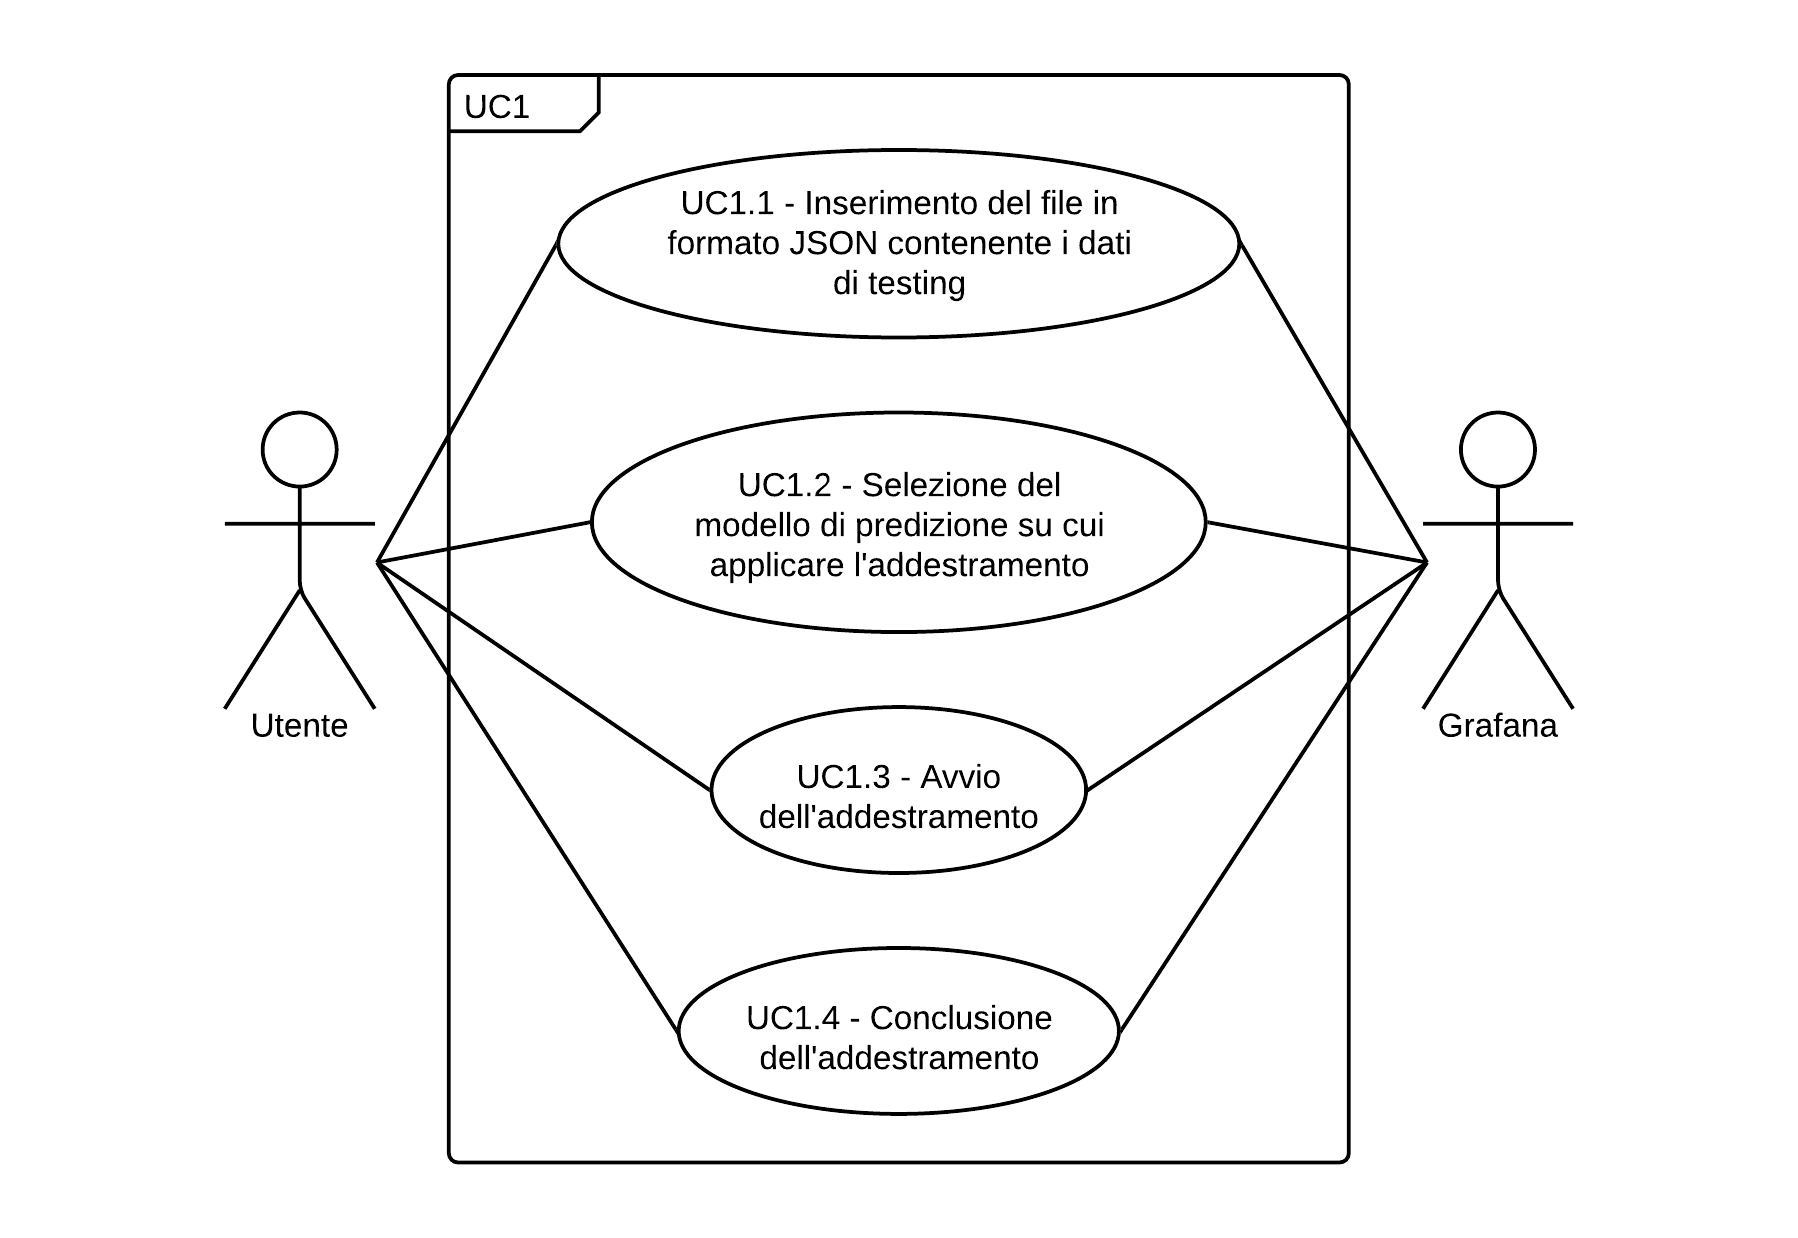
\includegraphics{img/UC1_-_Addestramento_degli_algoritmi_di_predizione_interno_a_Grafana.png}
\caption{Diagramma degli use case di UC1}
\end{figure}
\begin{itemize}
	\item \textbf{Codice identificativo}: UC1;
	\item \textbf{Titolo}: Addestramento degli algoritmi di predizione interno a Grafana\glo;
	\item \textbf{Attori primari}: Utente;
	\item \textbf{Attori secondari}: Grafana\glo;
	\item \textbf{Descrizione}: Attività di addestramento degli algoritmi di predizione interna a Grafana\glosp utilizzando dei dati inseriti da un utente autenticato;
	\item \textbf{Precondizioni}: L'utente è autenticato nel sistema software Grafana\glo;
	\item \textbf{Postcondizioni}: Grafana\glosp riceve i dati di predizione dopo l'addestramento dei dati caricati da utente;
	\item \textbf{Scenario principale}: 
		\begin{enumerate}
			\item Inserimento del file in formato JSON contenente i dati di testing (UC1.1);
			\item Selezione del modello di predizione su cui applicare l'addestramento (UC1.2);
			\item Avvio dell'addestramento (UC1.3);
			\item Conclusione dell'addestramento (UC1.4).
		\end{enumerate}
	\item \textbf{Estensioni}:
	\begin{itemize}
		\item Se il caricamento del file JSON non è avvenuto con successo viene visualizzato un messaggio di errore (UC3).
	\end{itemize}
\end{itemize}

\subsubsection{UC1.1 - Inserimento del file in formato JSON contenente i dati di testing}
\begin{figure}[H]
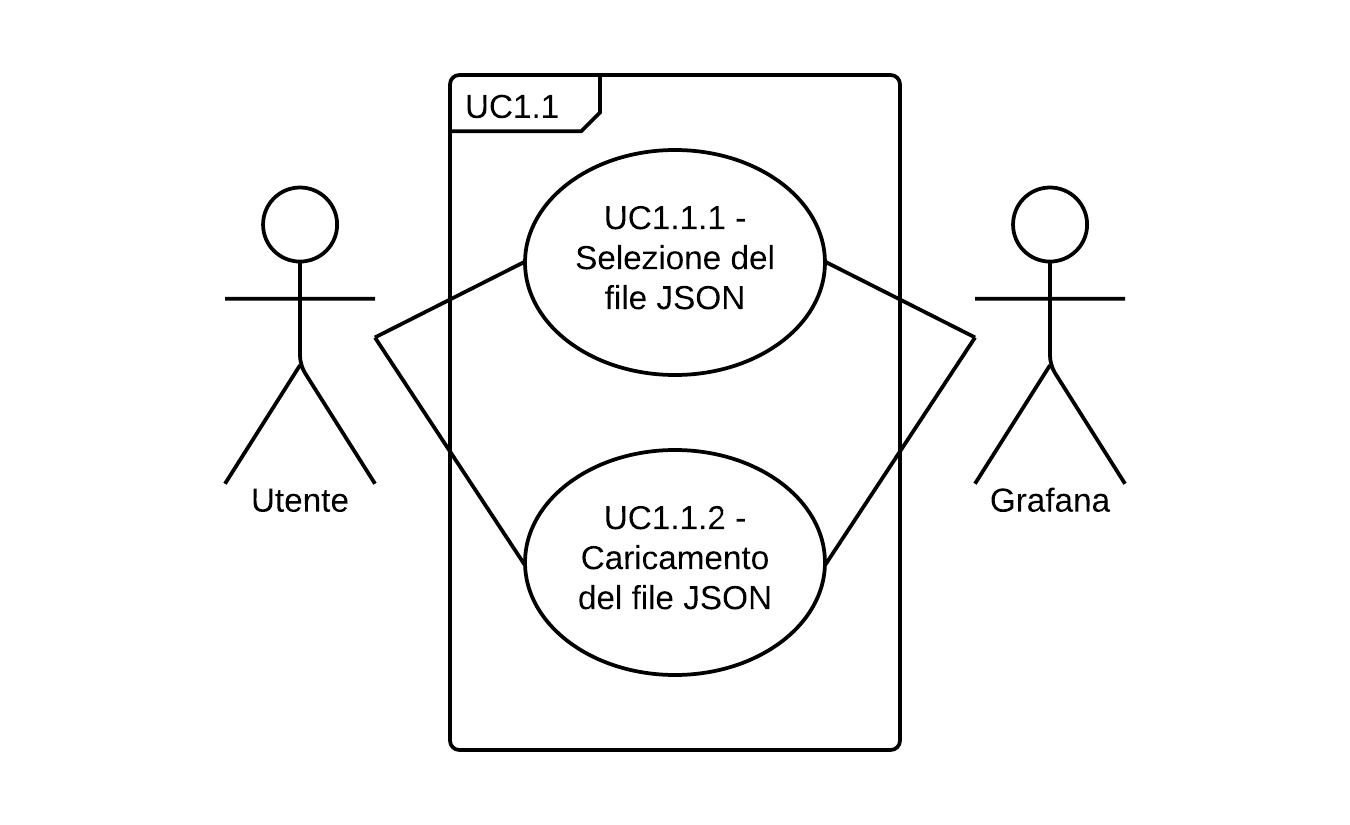
\includegraphics{img/UC1_1_-_Inserimento_del_file_in_formato_JSON_contenente_i_dati_di_testing.png}
\caption{Diagramma degli use case di UC1.1}
\end{figure}
\begin{itemize}
	\item \textbf{Codice identificativo}: UC1.1;
	\item \textbf{Titolo}: Inserimento del file in formato JSON contenente i dati di testing;
	\item \textbf{Attori primari}: Utente;
	\item \textbf{Attori secondari}: Grafana\glo;
	\item \textbf{Descrizione}: L'utente inserisce nel sistema di Grafana\glosp il file JSON che contiene dati di testing per l'addestramento degli algoritmi di predizione;
	\item \textbf{Precondizioni}: L'utente è autenticato nel sistema software Grafana\glo;
	\item \textbf{Postcondizioni}: Il file JSON contenente i dati di testing è stato inserito correttamente;
	\item \textbf{Scenario principale}:
		\begin{enumerate}
			\item Selezione del file JSON (UC1.1.1);
			\item Caricamento del file JSON (UC1.1.2).
		\end{enumerate}
\end{itemize}

\paragraph{UC1.1.1 - Selezione del file JSON}
\begin{itemize}
	\item \textbf{Codice identificativo}: UC1.1.1;
	\item \textbf{Titolo}: Selezione del file JSON;
	\item \textbf{Attori primari}: Utente;
	\item \textbf{Attori secondari}: Grafana\glo;
	\item \textbf{Descrizione}: L'utente seleziona il file JSON da inserire nel sistema;
	\item \textbf{Precondizioni}: L'utente è autenticato nel sistema software Grafana\glo;
	\item \textbf{Postcondizioni}: Il file JSON è stato selezionato correttamente;
	\item \textbf{Scenario principale}: L'utente seleziona il file JSON.
\end{itemize}

\paragraph{UC1.1.2 - Caricamento del file JSON}
\begin{itemize}
	\item \textbf{Codice identificativo}: UC1.1.2;
	\item \textbf{Titolo}: Caricamento del file JSON;
	\item \textbf{Attori primari}: Utente;
	\item \textbf{Attori secondari}: Grafana\glo;
	\item \textbf{Descrizione}: L'utente carica il file JSON selezionato;
	\item \textbf{Precondizioni}: L'utente autenticato ha selezionato il file JSON da caricare;
	\item \textbf{Postcondizioni}: Il file JSON è stato caricato correttamente;
	\item \textbf{Scenario principale}: L'utente carica del file JSON.
\end{itemize}

\subsubsection{UC1.2 - Selezione del modello di predizione su cui applicare l'addestramento}
\begin{itemize}
	\item \textbf{Codice identificativo}: UC1.2;
	\item \textbf{Titolo}: Selezione del modello di predizione su cui applicare l'addestramento;
	\item \textbf{Attori primari}: Utente;
	\item \textbf{Attori secondari}: Grafana\glo;
	\item \textbf{Descrizione}: L'utente seleziona quale modello di predizione applicare durante l'addestramento;
	\item \textbf{Precondizioni}: Il file JSON è stato inserito correttamente;
	\item \textbf{Postcondizioni}: L'utente ha selezionato correttamente il modello di predizione;
	\item \textbf{Scenario principale}: L'utente seleziona un modello di predizione per eseguire l'addestramento.
\end{itemize}

\subsubsection{UC1.3 - Avvio dell'addestramento}
\begin{itemize}
	\item \textbf{Codice identificativo}: UC1.3;
	\item \textbf{Titolo}: Avvio dell'addestramento;
	\item \textbf{Attori primari}: Utente;
	\item \textbf{Attori secondari}: Grafana\glo;
	\item \textbf{Descrizione}: L'utente avvia l'addestramento dei dati;
	\item \textbf{Precondizioni}: Il file JSON è stato inserito correttamente e il modello di predizione è stato selezionato;
	\item \textbf{Postcondizioni}: L'addestramento è stato avviato con successo;
	\item \textbf{Scenario principale}: L'utente avvia l'addestramento.
\end{itemize}

\subsubsection{UC1.4 - Conclusione dell'addestramento}
\begin{figure}[H]
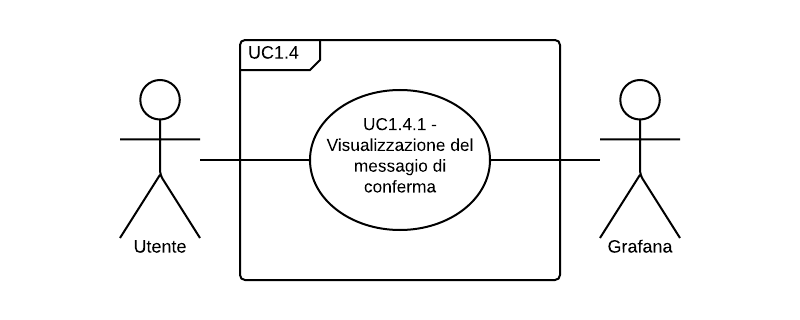
\includegraphics{img/UC1_4.png}
\caption{Diagramma degli use case di UC1.4}
\end{figure}
\begin{itemize}
	\item \textbf{Codice identificativo}: UC1.4;
	\item \textbf{Titolo}: Conclusione dell'addestramento;
	\item \textbf{Attori primari}: Utente;
	\item \textbf{Attori secondari}: Grafana\glo;
	\item \textbf{Descrizione}: L'addestramento è concluso;
	\item \textbf{Precondizioni}: L'addestramento è stato avviato con successo;
	\item \textbf{Postcondizioni}: L'addestramento è stato concluso con successo;
	\item \textbf{Scenario principale}: L'utente visualizza un messaggio di conferma e conclude l'addestramento.
\end{itemize}

\paragraph{UC1.4.1 - Visualizzazione del messaggio di conferma}
\begin{itemize}
	\item \textbf{Codice identificativo}: UC1.4.1;
	\item \textbf{Titolo}: Visualizzazione del messaggio di conferma;
	\item \textbf{Attori primari}: Utente;
	\item \textbf{Attori secondari}: Grafana\glo;
	\item \textbf{Descrizione}: L'utente visualizza un messaggio di conferma che l'addestramento è stato eseguito correttamente;
	\item \textbf{Precondizioni}: L'addestramento è stato avviato con successo;
	\item \textbf{Postcondizioni}: L'utente ha visualizzato un messaggio di conferma che l'addestramento è stato eseguito correttamente;
	\item \textbf{Scenario principale}: L'utente visualizza un messaggio di conferma che l'addestramento è stato eseguito correttamente.
\end{itemize}
